\section{Patterns 9 - Redegør for følgende concurrency mønstre}

\subsection{Fokuspunkter}

\begin{itemize}
	\item Futures.
	\item Pipelines.
\end{itemize}

\subsection{Future}
Vi starter ud med lidt om \textbf{dependancies}:

Afhængigheder er et problem for parallelisering.
Vi sorterer det der kan paralleliseres og gør det!

\begin{figure}[h]
\centering
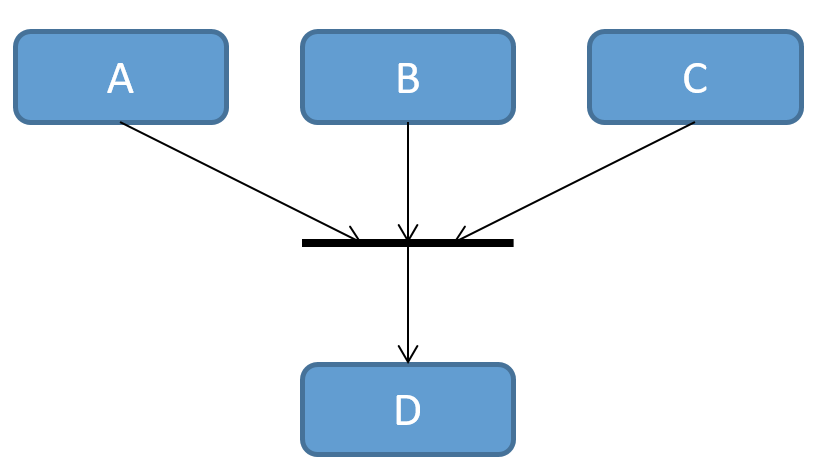
\includegraphics[width=0.5\linewidth]{figs/pipeFut/dependancies.PNG}
\caption{Node D skal køres før A, B og C kan køres parallelt}
\label{fig:dependancies}
\end{figure}

En future kan betegnes som en stand-in for en værdi der som udgangspunkt er utilgængelig, men som bliver tilgængelig på et senere tidspunkt.
Altså bruges futures når vi ønsker at parallelisere kode der har data dependancies.

\begin{figure}[h]
	\centering
	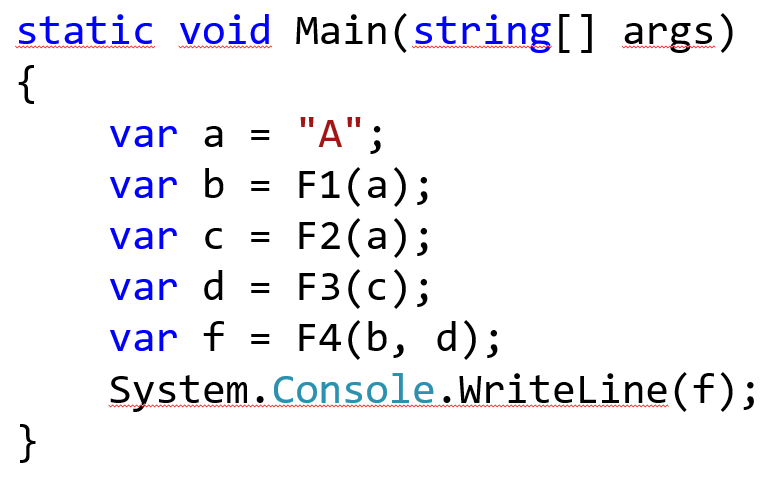
\includegraphics[width=0.5\linewidth]{figs/pipeFut/parallelThis.PNG}
	\caption{Data dependancies}
	\label{fig:Datadependancies}
\end{figure}

Vi laver en dependancy til en future! Altså et løfte om at den kommer!

\begin{figure}[H]
	\centering
	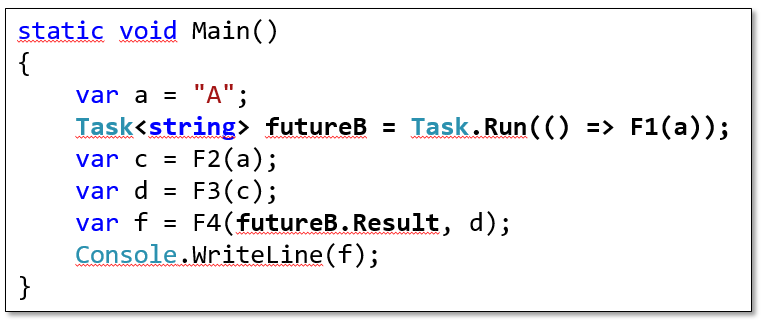
\includegraphics[width=0.6\linewidth]{figs/pipeFut/futureB}
	\caption{Brug af Futures}
	\label{fig:FutureEx}
\end{figure}

Forskellen mellem futures og parallel tasks er at \textbf{Futures} er asynkrone funktioner der \textbf{returnerer} en værdi, hvorimod Parallel tasks \textbf{ikke returnerer} en værdi.

\subsubsection{Fordele og ulemper}

Man undgår at en funktion får et forkert input fordi en anden funktion ikke er færdig.

På den anden side er det den langsomste funktion der afgør hastigheden på den samlede udførselstid.

\subsection{Pipelines}
\begin{itemize}
	\item Pipeline mønstret paralleliserer processeringen af en input sekvens.
	\item Pipeline mønstret består af en serie af producer/consumere.
	\item Opdeler processering i paralelliserbare stadier.
	\begin{itemize}
		\item Output af stage i er indput i stage i + 1:
		\item Andre stadier er uafhængige.
	\end{itemize}
\end{itemize}

Som det kan ses på figur \ref{fig:pipelining} har vi pipelinet processeringen af $C_1, C_2, C_3$ og $C_4$ 

\begin{figure}[H]
	\centering
	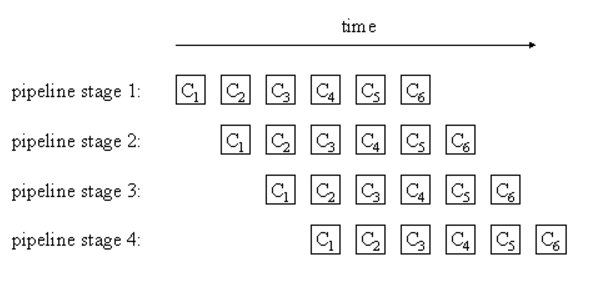
\includegraphics[width=0.7\linewidth]{figs/pipeFut/stagees}
	\caption{Brug af pipelining}
	\label{fig:pipelining}
\end{figure}

Man kunne forestille sig at et enkelt stage vill tage længere tid end de andre (uneven stage duration).

\begin{figure}[H]
	\centering
	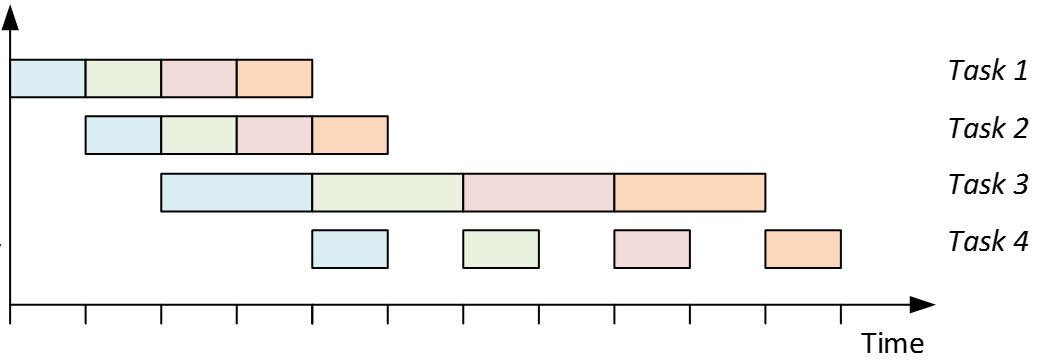
\includegraphics[width=0.7\linewidth]{figs/pipeFut/unevenStage}
	\caption{Standard pipelining med uneven stages}
	\label{fig:Unevenpipelining}
\end{figure}

Løsningen på dette problem er at tilføje en ekstra stage 3

\begin{figure}[H]
	\centering
	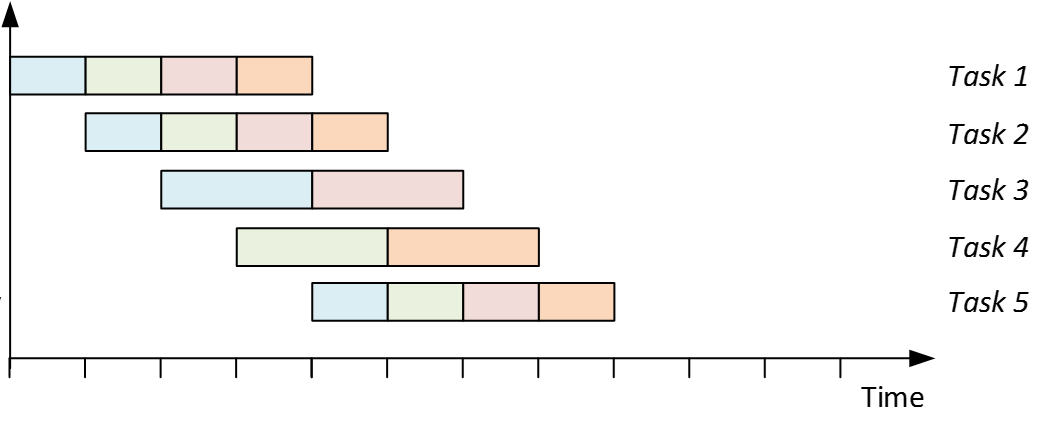
\includegraphics[width=0.7\linewidth]{figs/pipeFut/ekstraFilter}
	\caption{Pipelining med uneven stages + Ekstra stage}
	\label{fig:UnevenpipeliningWStage}
\end{figure}

\subsubsection{Fordele og ulemper}

Pipelining kan fremskynde processering der har flere stages.

Det er dog værd at bemærke  at pipelining ikke fremskynder den enkelte process, men derimod sikrer et større througput. Hvis pipelining ikke er nædbendigt, kræver det blot flere ressourcer.